\documentclass[14pt]{extarticle}
\usepackage{amsmath}
\usepackage{amssymb}
\usepackage{gvv}
\usepackage{bm}
\usepackage{graphicx}
\title{\textbf{5.3.39}}
\author{\textbf{Aditya Mishra-EE25BTECH11005}}
\date{October 3, 2025}

\begin{document}
\maketitle

\section*{Question}
Using matrices, solve the following system of equations:
\begin{align*}
    x + y + z &= 6 \\
    x + 2z &= 7 \\
    3x + y + z &= 12 
\end{align*}

\section*{Solution}
Forming the augmented matrix,
\[
\left(
\begin{array}{ccc|c}
1 & 1 & 1 & 6 \\
1 & 0 & 2 & 7 \\
3 & 1 & 1 & 12 \\
\end{array}
\right)
\]

Perform row operations to reduce to row echelon form:
\[
\left(
\begin{array}{ccc|c}
1 & 1 & 1 & 6 \\
1 & 0 & 2 & 7 \\
3 & 1 & 1 & 12 \\
\end{array}
\right)
\xrightarrow{R_2 \rightarrow R_2 - R_1}
\left(
\begin{array}{ccc|c}
1 & 1 & 1 & 6 \\
0 & -1 & 1 & 1 \\
3 & 1 & 1 & 12 \\
\end{array}
\right)
\]
\[
\xrightarrow{R_3 \rightarrow R_3 - 3R_1}
\left(
\begin{array}{ccc|c}
1 & 1 & 1 & 6 \\
0 & -1 & 1 & 1 \\
0 & -2 & -2 & -6 \\
\end{array}
\right)
\]
\[
\xrightarrow{R_3 \rightarrow R_3 - 2R_2}
\left(
\begin{array}{ccc|c}
1 & 1 & 1 & 6 \\
0 & -1 & 1 & 1 \\
0 & 0 & -4 & -8 \\
\end{array}
\right)
\]

From the third row:
\[
-4z = -8 \implies z = 2
\]
From the second row:
\[
-y + z = 1 \implies -y + 2 = 1 \implies y = 1
\]
From the first row:
\[
x + y + z = 6 \implies x + 1 + 2 = 6 \implies x = 3
\]

Thus, the solution is :
\[
\boxed{
\vec{x} = \myvec{3 \\ 1 \\ 2}
}
\]
\newpage
\section*{Plot}
\begin{figure}[!h]
    \centering
    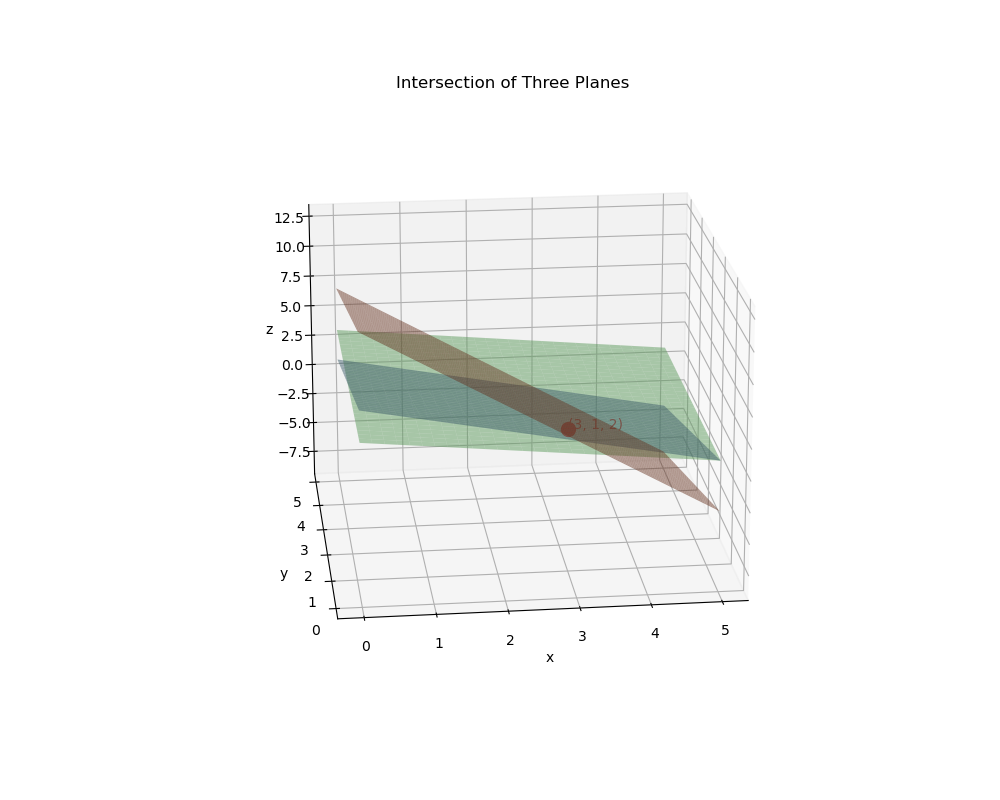
\includegraphics[width=1.2\columnwidth]{Figs/Figure_1.png}
\end{figure}
\end{document}

